\documentclass[letterpaper,12pt]{report}
\usepackage{thesis}
\usepackage{float}
\usepackage[hyphens]{url}            % para partir URLs largas
\usepackage{graphicx}
\usepackage{latexsym}
\usepackage{rotating}
\usepackage{natbib} 
\usepackage[expansion=false]{microtype}
\usepackage{array}
\usepackage{tabularx}                 
\usepackage[colorlinks=true,linkcolor=black,citecolor=black]{hyperref} % cargar al final si no hay paquetes muy especiales
% Cambiar nombres de capítulos y secciones al español
\renewcommand{\chaptername}{Capítulo}
\renewcommand{\contentsname}{Índice general}
\renewcommand{\listfigurename}{Índice de figuras}
\renewcommand{\listtablename}{Índice de tablas}
\renewcommand{\bibname}{Bibliografía}
\renewcommand{\appendixname}{Apéndice}
\renewcommand{\figurename}{Figura}
\renewcommand{\tablename}{Tabla}
\renewcommand{\abstractname}{Resumen}
\renewcommand{\indexname}{Índice alfabético}
\renewcommand{\partname}{Parte}
\renewcommand{\bibname}{Referencias}
\renewcommand{\refname}{Referencias}

\begin{document}

\pagenumbering{roman}

% Fill in the title, author, degree name, department, and month/year.
% Upon completion, this should look like the following:
%\thesistitle
%	{Complicated and Important-Sounding Thesis Title}
%	{John P. Doe}
%	{Master of Science}
%	{Department of Computer Science}
%	{May 2009}
% The \thesistitle definition is in thesis.sty.  Other customizations
% can be made there.

\thesistitle
    {Proyecto de Curso: \\ 
     Análisis, Diseño y Construcción de un Sistema Operativo desde Cero}
    {Castro Pari, Rayneld Fidel \\ 
     Mamani Flores, Natan \\ 
     Mendoza Quispe, Jose Daniel \\ 
     Polo Chura, Marco Rosauro}
    {Proyecto de Investigación de la Primera Unidad de Sistemas Operativos \\
    % --- Logos ---
    \begin{minipage}{0.45\textwidth}
        \centering
        
\includegraphics[width=0.8\linewidth]{figures/UNSAAC.png}
    \end{minipage}%
    \hfill
    \begin{minipage}{0.45\textwidth}
        \centering
        
\includegraphics[width=0.8\linewidth]{figures/INGINFO.jpg}
    \end{minipage}
    }
    {Departamento Académico de Ingeniería de Informatica y de Sistemas \\ 
     Asesor: Ugarte Rojas, Héctor Eduardo}
    {Semestre 2025-II}
\tableofcontents
\clearpage
\phantomsection   
\addcontentsline{toc}{chapter}{Índice de tablas}
\listoftables

\clearpage
\phantomsection   
\addcontentsline{toc}{chapter}{Índice de figuras}
\listoffigures


\pagenumbering{arabic}
\chapter*{Introduccion}
\addcontentsline{toc}{chapter}{Introducción}

El desarrollo y la transformación de los sistemas operativos han sido fundamentales en la evolución de las tecnologías de la información. Desde los primeros programas creados para las computadoras centrales hasta los sistemas más utilizados en ordenadores personales, dispositivos móviles y equipos embebidos, los sistemas operativos han actuado como un puente entre las necesidades del usuario y la complejidad del hardware. Estudiarlos no solo permite entender el funcionamiento básico de una computadora, sino que también brinda las bases conceptuales y técnicas necesarias para el diseño de nuevas soluciones informáticas. Este documento tiene como finalidad ofrecer una perspectiva global de los sistemas operativos, abordando sus características principales, su arquitectura y sus componentes.

\section*{Objetivo de la investigacion}

El objetivo principal de este trabajo es realizar un análisis técnico y comparativo de distintos sistemas operativos, con la finalidad de identificar sus características más relevantes y examinar las diversas concepciones y enfoques aplicados en su diseño e implementación. Se estudiarán tanto arquitecturas tradicionales, como la monolítica, así como modelos más modernos, entre ellos los exokernels, híbridos y microkernels . Del mismo modo, se pretende ofrecer una visión crítica sobre las ventajas, limitaciones y ámbitos de aplicación de cada sistema operativo.

\section*{Alcance del análisis}
El presente estudio se centra en sistemas operativos ampliamente utilizados y representativos de diferentes enfoques arquitectónicos y áreas de aplicación. No se abordarán sistemas altamente experimentales o versiones obsoletas a menos que sean relevantes para la comparación histórica o conceptual. El análisis incluye tanto sistemas de propósito general (Windows, macOS, Linux) como sistemas especializados (RTOS, embebidos y móviles), enfocándose en aspectos técnicos, operativos y comunitarios que permitan identificar fortalezas, limitaciones y escenarios de uso recomendados para cada sistema operativo.

\section*{Metodologia}

Con el fin de alcanzar los objetivos planteados, se seguirá una metodología compuesta por tres fases fundamentales:

\begin{enumerate}
\item \textbf{Revisión bibliográfica y documental:} Se consultarán libros especializados, artículos académicos, blogs técnicos, documentación oficial y repositorios relacionados con los sistemas operativos en estudio.

\item \textbf{Evaluación técnica:} Se examinarán los aspectos esenciales de cada sistema, incluyendo la gestión de procesos, la administración de memoria, los sistemas de archivos, el manejo de dispositivos, las interfaces de usuario y los mecanismos de seguridad.  

\item \textbf{Comparación estructurada:} Se elaborará una tabla que sintetice las características más representativas de los sistemas operativos analizados, tomando en cuenta factores como el tamaño del kernel, la arquitectura, la comunidad, el lenguaje de implementación, la documentación disponible y el soporte de hardware.  


\end{enumerate}

Este enfoque permitirá garantizar un análisis más objetivo, completo y útil, tanto para fines académicos como prácticos.


\chapter{Marco teórico}
\section{¿Que es un sistema operativo?}
Según Stallings, el sistema operativo es el software encargado de controlar 
la ejecución de los programas y de administrar los recursos del procesador; 
además actúa como intermediario entre el usuario y el hardware, proporcionando
los servicios necesarios para que las aplicaciones puedan ejecutarse correctamente \citep{Stallings2023} 

Añadiendo esta idea, Tanenbaum y Bos explican que la finalidad del sistema 
operativo es convertir las interfaces de hardware, que suelen ser complejas e 
inconsistentes, en abstracciones practicas y sencillas de usar para los programadores
y aplicaciones. Ademas de gestionar recursos como CPU, memoria y dispositivos de E/S, permitiendo así
que las aplicaciones trabajen sin problemas con el hardware \citep{Tanenbaum2023}.

Según el artículo de la Revista Ogma, que es un científica y multidisciplinaria, un 
sistema operativo es el software principal que actúa como intermediario 
entre el usuario y el hardware, cuyo propósito es favorecer el uso eficiente 
de la computadora. Transforma las interfaces de hardware, complejas e inconsistentes, en abstracciones útiles y manejables para 
y aplicaciones y programadores, administra y mejora recursos (CPU, memoria, 
dispositivos de E/S y almacenamiento); organiza la ejecución concurrente de 
tareas, y ofrece espacios accesibles que permite el acceso de las 
computadoras, permitiendo que usuarios sin preparación instalen 
programas, administren archivos. \citep{CusmeVera2022}

Un sistema operativo es como el sistema nervioso del computador, coordinando 
componentes hardware y software para que todo funcione de manera ordenada. Se 
encarga de organizar y administrar recursos como procesador, memoria, 
dispositivos de E/S y almacenamiento.

\section{Tipos de sistemas operativos}
Los sistemas operativos pueden clasificarse de diversas maneras, por la administración de usuarios, administración de tareas, manejo de recursos, entorno de destino, entre otros criterios. En esta sección se abordarán específicamente las siguientes clasificaciones: sistemas operativos monousuario y multiusuario, monotarea y multitarea, de tiempo real (RTOS), distribuidos, móviles y embebidos. A continuación, el análisis de dichas clasificaciones.

\subsection{Monousuario vs. Multiusuario}
Estos tipos de sistemas operativos, son resultado de una clasificación por la cantidad de usuarios que los operan.  

\textbf{Monousuario:} Como su nombre hace evidente, fue planificado para usar la computadora de forma que solo una persona a la vez lo haga correctamente, esto no significa necesariamente que solo pueda hacer una tarea a la vez \citep{kaur2022osreview}. Sin embargo y completando el concepto, en la práctica más de una persona puede usarlo debido a que el sistema operativo no distingue entre personas \citep{olivares2021sohardware}. Según \citep{kaur2022osreview}, algunos ejemplos resaltantes de sistemas operativos monousuario son Palm OS y Windows (versiones antiguas).  

\textbf{Multiusuario:} Este tipo de sistema, hace posible que varios usuarios usen el computador de manera simultánea, para lo cual el sistema operativo debe administrar los recursos de manera adecuada; es necesario distinguir sistemas operativos multiusuario de sistemas monousuario compatibles con redes, en los cuales el único usuario “real” es el administrador \citep{kaur2022osreview}; otra característica del tipo multiusuario es distinguir entre las personas (usuarios) que acceden a la computadora \citep{olivares2021sohardware}. Según \citep{kaur2022osreview} complementado por \citep{olivares2021sohardware} y \citep{kabiraj2018oscase}, algunos ejemplos resaltantes de sistemas operativos multiusuario son Windows 7, Windows 10, UNIX, LINUX, VMS y el sistema operativo de servidor MVS.  

\subsection{Monotarea vs. Multitarea}
Estos tipos de sistemas operativos, son resultado de una clasificación por la administración de la ejecución de tareas.  

\textbf{Monotarea:} Como indica su raíz griega, solo hacen una tarea a la vez. En la actualidad están casi en completo desuso, debido a que no aprovecha de manera óptima los recursos. Un ejemplo resaltante de sistema operativo multitarea es MS-DOS, el cual actualmente se encuentra en desuso \citep{olivares2021sohardware}.  

\textbf{Multitarea:} Estos sistemas operativos son capaces de ejecutar varias tareas a la vez, y por ello maximizan el uso de los recursos de la computadora. Además, también algunos sistemas operativos para móviles son multitarea. Los sistemas operativos multitarea, a su vez se pueden clasificar por su forma de administrar el tiempo de ejecución de sus aplicaciones en: Sistemas de tiempo compartido y sistemas de tiempo real \citep{olivares2021sohardware}. Según \citep{rawat2025osstudy} algunos ejemplos resaltantes de sistemas operativos multitarea son Windows 10/11, Linux, Unix, macOS.  

\subsection{Tiempo real (RTOS)}
Los sistemas operativos de tiempo real son un tipo de sistema operativo multitarea. Mientras que su contraparte, los sistemas de tiempo compartido, se aprovechan del uso de pequeños intervalos de tiempo, para asignarlos a la ejecución de cada programa (time slice) y cambiar rápidamente entre las ejecuciones de estos programas (context switch), dando así la sensación de paralelismo; los sistemas operativos de tiempo real, no poseen intervalos de tiempo para definir la ejecución de un programa, sino que el programa se ejecuta hasta que termine (y dicho tiempo está definido también en el programa) o hasta que un programa de mayor prioridad lo interrumpa \citep{olivares2021sohardware}.  

En la actualidad se usan mayormente los sistemas operativos de tiempo compartido, pero los sistemas operativos de tiempo real juegan un papel clave en campos que requieran precisión en cuanto al tiempo de procesamiento como medicina, tráfico aéreo, plantas de energía, entre otros \citep{olivares2021sohardware}.  

En síntesis, estos sistemas buscan precisión en la sincronización, a partir de respuestas predecibles (determinismo) y se pueden clasificar de acuerdo a su tolerancia a errores en RTOS duros y RTOS suaves. Algunos ejemplos resaltantes son VxWorks, FreeRTOS y QNX \citep{rawat2025osstudy}.  

\subsection{Distribuidos}
Los sistemas operativos distribuidos controlan múltiples nodos independientes como si fueran un solo sistema, varios computadores en red ejecutan conjuntamente un OS único, de modo que el usuario percibe una sola computadora con hardware extra. Cada nodo corre un núcleo mínimo y componentes de gestión que intercomunican y comparten recursos con el objetivo de lograr transparencia (single-system image) \citep{garg2013dos}. Algunos ejemplos resaltantes son Google Fuchsia OS y Solaris OS \citep{rawat2025osstudy}.  

\begin{figure}[H]
    \centering
    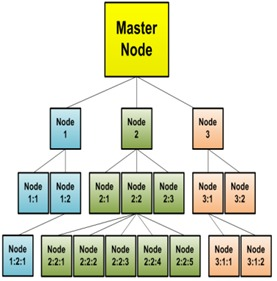
\includegraphics[width=0.4\textwidth]{figures/distributedSistems.jpg}
    \caption[Organización de nodos en un sistema operativo distribuido]%
            {Organización de nodos en un sistema operativo distribuido \citep{garg2013dos}}
    \label{fig:distributed_os}
\end{figure} 

\subsection{Móviles}
Los sistemas operativos móviles se diseñan para teléfonos inteligentes, tabletas y otros dispositivos portátiles táctiles, tiene como característica ser bastante intuitivos, ligeros y con un enfoque hacia el ahorro de la batería. Además, admiten funciones avanzadas en tecnología como interacción táctil, comunicación inalámbrica y ejecución de diversas aplicaciones. Algunos de los ejemplos más resaltantes son Android OS e iOS \citep{rawat2025osstudy}.  

A continuación, una línea de tiempo de la evolución de los sistemas operativos móviles:  

\begin{figure}[H]
    \centering
    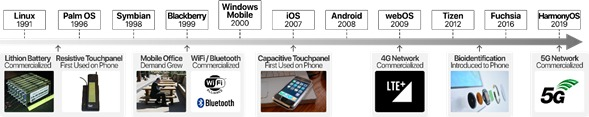
\includegraphics[width=1.0\textwidth]{figures/timeLineMobile.jpg}
    \caption[Desarrollo cronológico de los sistemas operativos móviles y hitos tecnológicos asociados]
            {Desarrollo cronológico de los sistemas operativos móviles y hitos tecnológicos asociados \citep{jia2024acos}}
    \label{fig:mobile_os}
\end{figure} 

\subsection{Embebidos}
Los sistemas operativos embebidos son diseñados para satisfacer los requerimientos específicos de los sistemas embebidos, son aplicados en diversos campos, tales como electrodomésticos, controles remotos e incluso instrumentos aeroespaciales. No requieren de demasiados recursos como energía, memoria ni espacio de almacenamiento; y aún así son capaces de brindar eficiencia y precisión, además de un nivel de personalización bastante alto para hacerlos funcionar en situaciones difíciles y cambiantes \citep{jia2024acos}. Algunos de los ejemplos más resaltantes son Embedded Linux y Windows Embedded Compact \citep{rawat2025osstudy}.  

A continuación, una línea de tiempo de la evolución de los sistemas operativos embebidos:  

\begin{figure}[H]
    \centering
    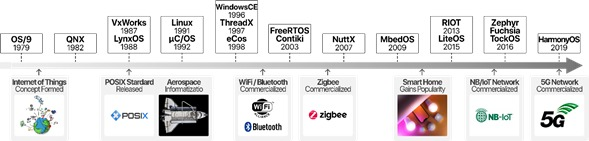
\includegraphics[width=1.0\textwidth]{figures/timeLineEmbeded.jpg}
    \caption[Desarrollo cronológico de los sistemas operativos embebidos y hitos tecnológicos asociados]
            {Desarrollo cronológico de los sistemas operativos embebidos y hitos tecnológicos asociados \citep{jia2024acos}}
    \label{fig:Embedded_os}
\end{figure} 

\subsection{Comparación entre tipos de Sistemas Operativos}

\begin{munltab}{|c|p{8cm}|p{8cm}|}
  {comparacion_tipos_so}
  {Comparación de tipos de sistemas operativos basado mayormente en \citep{rawat2025osstudy}}
\hline
\textbf{Tipo de SO} & \textbf{Ventajas} & \textbf{Desventajas} \\
\hline
Monousuario & Simplicidad en diseño y administración, adecuado para uso personal & No diferencia usuarios, limitaciones en entornos colaborativos \\
\hline
Multiusuario & Permite que múltiples usuarios accedan simultáneamente, gestión de recursos más avanzada & Mayor complejidad en seguridad y administración de cuentas \\
\hline
Monotarea & Implementación sencilla, bajo consumo de recursos & No aprovecha el hardware moderno, ineficiente y obsoleto \\
\hline
Multitarea & Aprovecha mejor los recursos, permite ejecución paralela de procesos & Complejidad en la gestión de concurrencia y planificación \\
\hline
Tiempo Real (RTOS) & Respuestas deterministas, precisión crítica en aplicaciones sensibles (medicina, aeroespacial, etc.) & Difícil de implementar, requiere hardware confiable y costoso \\
\hline
Distribuidos & Transparencia de recursos, escalabilidad, tolerancia a fallos & Complejidad en diseño, comunicación entre nodos y sincronización \\
\hline
Móviles & Interfaz intuitiva, eficiencia energética, portabilidad & Limitados en recursos frente a sistemas de escritorio, dependencia de ecosistema cerrado \\
\hline
Embebidos & Alta eficiencia y personalización, bajos requerimientos de hardware & Poco flexibles, difíciles de actualizar y mantener \\
\hline
\end{munltab}


\section{Arquitecturas de Sistemas Operativos}
\subsection{Arquitectura Monolítica}
El sistema operativo monolítico es un sistema operativo muy simple donde el núcleo controla directamente la gestión de dispositivos, memoria, archivos y procesos. Todos los recursos del sistema son accesibles al núcleo. En los sistemas monolíticos, cada componente del sistema operativo está contenido dentro del núcleo.\\
En una arquitectura monolítica, el núcleo del sistema operativo está diseñado para proporcionar todos los servicios del sistema operativo, incluyendo la gestión de memoria, la programación de procesos, los controladores de dispositivos y los sistemas de archivos, en un único y gran binario. Esto significa que todo el código se ejecuta en el espacio del núcleo, sin separación entre los procesos del núcleo y los del usuario \citep{geeks_monolithic}.


\begin{figure}[H]
    \centering
    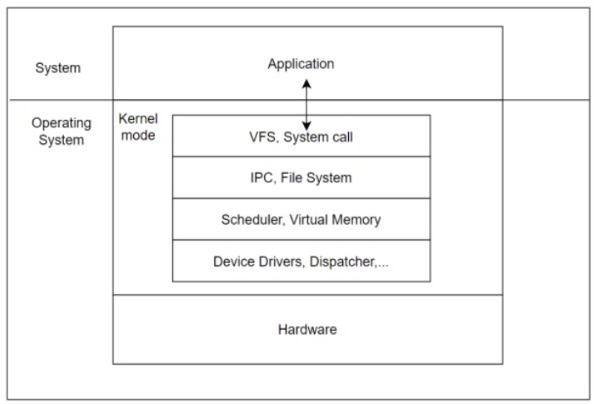
\includegraphics[width=0.7\textwidth]{figures/monolitica.jpeg}
    \caption[Sistema operativo basado en kernel monolítico]%
            {Sistema operativo basado en kernel monolítico \citep{harshvardhan2023kernels}}
    \label{fig:arquitectura_monolitica}
\end{figure}

\subsection{Arquitectura en Microkernel}
Un microkernel es un enfoque para diseñar un sistema operativo (SO). El microkernel proporciona servicios fundamentales para su funcionamiento, como la gestión básica de memoria, la programación de tareas.El microkernel es un tipo de sistema operativo que proporciona servicios básicos.\\
como los controladores de dispositivos y los sistemas de archivos, son gestionados por procesos a nivel de usuario. El proceso a nivel de usuario se comunica con el microkernel mediante el paso de mensajes. Esta forma de gestionar el proceso hace que los microkernels sean más modulares y flexibles que los kernels monolíticos tradicionales \citep{geeks_microkernel}.


\begin{figure}[H]
    \centering
    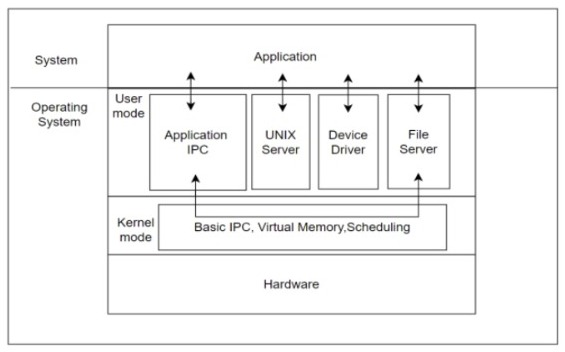
\includegraphics[width=0.7\textwidth]{figures/microkernel.jpeg}
    \caption[Sistema operativo basado en microkernel]%
            {Sistema operativo basado en microkernel \citep{harshvardhan2023kernels}}
    \label{fig:arquitectura_microkernel}
\end{figure}

\subsection{Arquitectura Hibrida}
Un núcleo híbrido es una arquitectura de núcleo basada en la combinación de aspectos de las arquitecturas de micronúcleo y núcleo monolítico utilizadas en sistemas operativos .\\
La idea de esta categoría es tener una estructura de kernel similar a la de un microkernel, pero implementada en términos de un kernel monolítico. A diferencia de un microkernel, todos (o casi todos) los servicios del sistema operativo se encuentran en el espacio del kernel . Si bien no hay sobrecarga de rendimiento para el paso de mensajes ni el cambio de contexto entre el kernel y el modo de usuario, como en los kernels monolíticos , no hay ventajas de rendimiento al tener servicios en el espacio de usuario , como en los microkernels \citep{ms_hybrid_kernel}.
\begin{figure}[H]
    \centering
    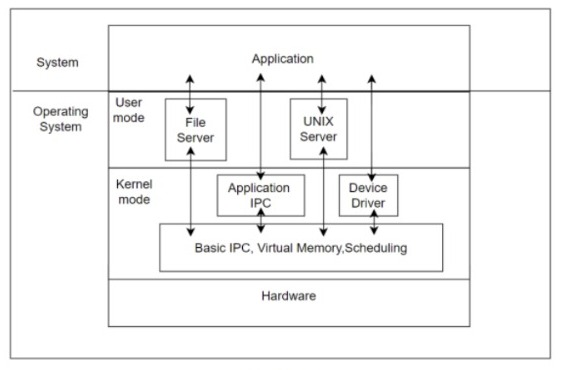
\includegraphics[width=0.7\textwidth]{figures/hibridokernel.jpeg}
    \caption[Sistema operativo basado en kernel híbrido]%
            {Sistema operativo basado en kernel híbrido \citep{harshvardhan2023kernels}}
    \label{fig:arquitectura_kernel_hibrido}
\end{figure}


\subsection{Arquitectura en Exokernel}
Exokernel es un sistema operativo desarrollado por el Instituto Tecnológico de Massachusetts (MIT) con el concepto de poner la aplicación bajo control. Los sistemas operativos Exokernel buscan proporcionar gestión de recursos de hardware a nivel de aplicación. La arquitectura de este sistema operativo está diseñada para separar la protección de recursos de la gestión, facilitando así la personalización específica de cada aplicación\citep{keetmalin2017exokernel}.




\begin{figure}[H]
    \centering
    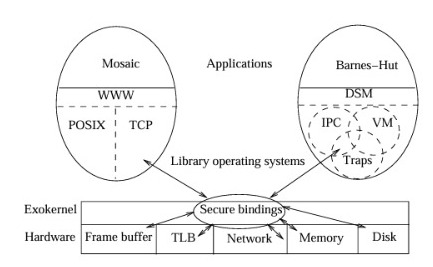
\includegraphics[width=0.7\textwidth]{figures/hexokernel.jpeg}
    \caption[Sistema operativo basado en exokernel]%
            {Sistema operativo basado en exokernel \citep{exokernel1995}}
    \label{fig:arquitectura_kernel_exokernel}
\end{figure}



\subsection{Comparacion entre arquitecturas de Sistemas Operativos}

\begin{muntab}{|c|p{5cm}|p{5cm}|}
  {comparacion_kernel}
  {Comparación de arquitecturas de SO basado mayormente en \citep{harshvardhan2023kernels}}
\hline
\textbf{Arquitectura} & \textbf{Ventajas} & \textbf{Desventajas} \\
\hline
Monolítica & Alto rendimiento, simple en diseño inicial & Difícil de mantener, poco modular \\
\hline
Microkernel & Modularidad, mayor seguridad & Mayor sobrecarga de comunicación \\
\hline
Hibrida & Combina rendimiento y modularidad & Complejidad de implementacion \\
\hline
Exokernel & Máxima flexibilidad y control & Muy complejo, poco usado en producción \\
\hline
\end{muntab}

\section{Componentes principales de un sistema operativo}

Un sistema operativo integra diversos componentes que gestionan los recursos de hardware y ofrecen servicios a los procesos que se ejecutan en el sistema.  

\subsection{Gestión de procesos}

La gestión de procesos es uno de los pilares fundamentales de cualquier sistema operativo, ya que se encarga de controlar la ejecución de programas y de garantizar un uso eficiente de la CPU. Un proceso, desde su creación hasta su finalización, pasa por diferentes estados a lo largo de su ciclo de vida. Al crearse, entra en el estado nuevo; luego pasa al estado preparado mientras espera acceso a la CPU. Cuando el planificador lo selecciona, pasa a ejecutando. Durante la ejecución, un proceso puede quedar en espera si requiere operaciones de entrada/salida, y finalmente alcanza el estado terminado al completar su tarea, como se muestra en la Figura \ref{fig:ciclo_vida_proceso}.  

\begin{figure}[H]
    \centering
    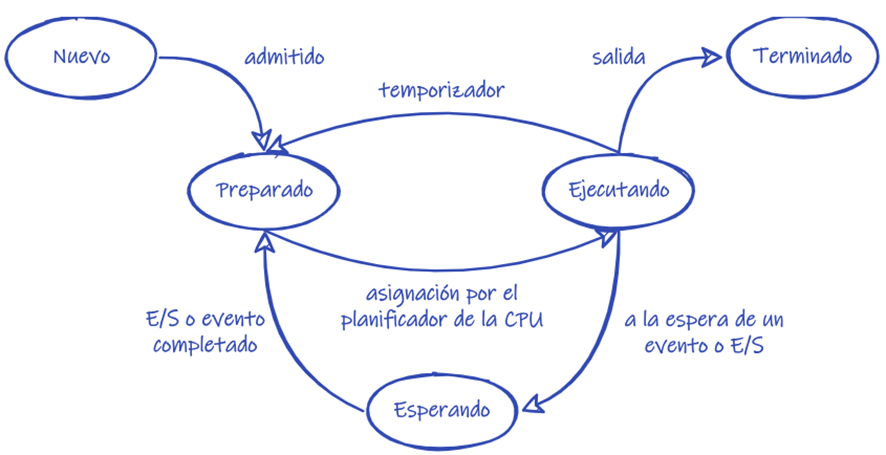
\includegraphics[width=0.7\textwidth]{figures/ciclo_vida_proceso.png}
    \caption[Diagrama de estados de un proceso]%
            {Diagrama de estados de un proceso. Fuente: \citep{torres2024}}
    \label{fig:ciclo_vida_proceso}
\end{figure}

Entre las funciones principales de la gestión de procesos se encuentra la creación y finalización de procesos. El sistema operativo se encarga de iniciar nuevos procesos mediante llamadas al sistema (por ejemplo, \texttt{fork} en Unix) y de eliminar aquellos que ya han concluido su ejecución \citep{juan2015}.  

Otra función esencial es la planificación o \textit{scheduling}, que consiste en decidir el orden en el que los procesos acceden a la CPU. Para ello se emplean algoritmos como FIFO, round robin o planificación basada en prioridades, según los objetivos de rendimiento y equidad del sistema \citep{juan2015}.  

Asimismo, la gestión de procesos incluye mecanismos de sincronización y comunicación, conocidos como IPC (Inter-Process Communication). Estos permiten que los procesos se coordinen y compartan información de manera segura, evitando condiciones de carrera y conflictos al acceder a recursos comunes \citep{wikipedia}.  
\newpage
\begin{muntab}{|p{4cm}|p{9cm}|}
  {razones_creacion_procesos}
  {Razones comunes para la creación de procesos en un sistema operativo \citep{sistemas_operativos}}
\hline
\textbf{Tipo de proceso} & \textbf{Descripción} \\
\hline
Proceso por lotes & El SO procesa trabajos en lote desde cinta/disco. Lee secuencias de control de trabajos automáticamente. \\
\hline
Sesión interactiva & Usuario inicia sesión desde un terminal. \\
\hline
Servicio del sistema & El SO crea procesos para servicios en segundo plano (ej: impresión) sin espera del usuario. \\
\hline
Proceso hijo & Proceso existente crea nuevos procesos para modularidad o paralelismo. \\
\hline
\end{muntab}
\newpage
\begin{muntab}{|p{4cm}|p{10cm}|}
  {razones_terminacion}
  {Razones comunes para la terminación de procesos en un sistema operativo \citep{sistemas_operativos}}
\hline
\textbf{Causa de terminación} & \textbf{Descripción} \\
\hline
Finalización normal & Completación voluntaria mediante llamada al sistema. \\
\hline
Límite de tiempo & Exceso de tiempo de ejecución o espera. \\
\hline
Memoria no disponible & Memoria insuficiente o acceso no permitido. \\
\hline
Error de protección & Uso no autorizado de recursos. \\
\hline
Error aritmético & Operación inválida (ej: división por cero). \\
\hline
Fallo de E/S & Error en operación de entrada/salida. \\
\hline
Instrucción inválida & Ejecución de instrucción inexistente. \\
\hline
Instrucción privilegiada & Uso de instrucción reservada al SO. \\
\hline
Datos inapropiados & Datos erróneos o no inicializados. \\
\hline
Intervención externa & Terminación por operador o SO. \\
\hline
Terminación por padre & Finalización por proceso padre (automática o solicitada). \\
\hline
\end{muntab}
\newpage
\subsection{Gestión de memoria}

La gestión de memoria es esencial para que el sistema operativo asigne y libere espacio en la memoria principal (RAM) a los procesos en ejecución. Su función principal consiste en aislar los espacios de direcciones de cada programa, de modo que puedan ejecutarse de manera concurrente sin interferir entre sí. Gracias a este control, la CPU puede cargar en memoria las instrucciones y datos necesarios de cada proceso en el momento oportuno. En términos generales, el administrador de memoria organiza los procesos de tal manera que se obtenga la máxima utilidad del espacio disponible, trasladando a la memoria principal la información que debe ejecutarse en cada instante \citep{wikipedia1}.  

En los sistemas modernos esta gestión se fundamenta en el concepto de memoria virtual, que proporciona a cada proceso una memoria lógica mayor que la memoria física disponible. Para ello se emplean técnicas como la paginación, en las que cada proceso dispone de su propia tabla de páginas que mapea direcciones lógicas hacia marcos de la memoria física. En la Figura \ref{fig:memoria} se ilustra este esquema, donde las páginas virtuales de los procesos se corresponden con bloques de memoria física compartida de manera ordenada.  

\begin{figure}[H]
    \centering
    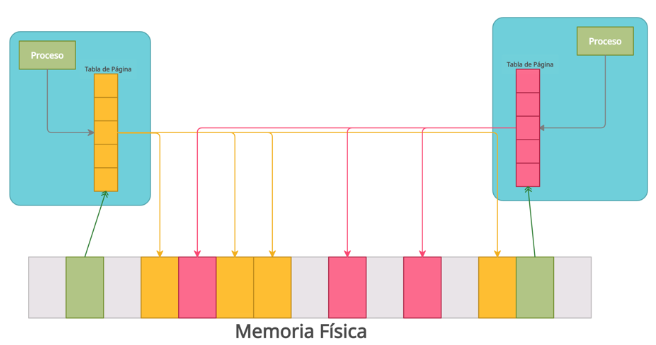
\includegraphics[width=0.8\textwidth]{figures/memoria.png}
    \caption{Traducción por paginación. Cada proceso (cajas turquesa) posee su propia tabla de páginas (columnas amarilla y rosada) que asigna páginas lógicas a marcos de la memoria física (bloques coloreados). Fuente: \citep{wikipedia2}}
    \label{fig:memoria}
\end{figure}

Entre las funciones principales del gestor de memoria se encuentran el control del uso de la memoria, la asignación y liberación de espacio para los procesos, la reubicación de datos en caso necesario, la gestión de la fragmentación y la compactación, la implementación de la memoria virtual y la protección de los espacios de direcciones para evitar accesos indebidos entre procesos. Estas tareas en conjunto garantizan un uso eficiente y seguro del recurso más limitado y compartido del sistema.  

La traducción mediante paginación, como se aprecia en la figura, permite que cada proceso perciba su espacio de direcciones como contiguo, aunque en la práctica las páginas estén distribuidas en diferentes marcos físicos de la RAM. El sistema operativo se encarga de mantener actualizadas las tablas de páginas y, cuando es necesario, puede intercambiar páginas entre la memoria principal y el disco, asegurando así la abstracción de una memoria virtual continua \citep{ucm2020}.  
\subsection{Sistema de archivos}

\subsubsection{Estructura jerárquica}
El sistema de archivos organiza los archivos y directorios en forma de árbol invertido. A nivel lógico existe un único directorio raíz (/), 
nodo principal que contiene todos los demás. Cada nodo del árbol corresponde a un directorio que puede contener subdirectorios, archivos normales o especiales.
Este diseño jerárquico con nombres únicos por directorio facilita la navegación y la gestión, evitando colisiones de nombres.

\subsubsection{Gestión de datos persistentes}
El sistema de archivos provee los medios para almacenar y recuperar datos de forma ordenada en la memoria secundaria (discos, SSD, etc.). 
La memoria se divide en bloques de tamaño fijo, y el sistema de archivos asigna a cada archivo los bloques necesarios. 
Además, controla la consistencia de los datos mediante técnicas como journaling, asegurando que la información persista aunque finalicen los procesos o falle el sistema. 
También gestiona la integridad ante fallos, permitiendo recuperar estructuras de disco sin pérdida de datos~\citep{ual2019}.

\subsubsection{Operaciones de archivo}
El sistema de archivos ofrece llamadas básicas para crear, abrir, leer, escribir, renombrar y eliminar archivos y directorios. 
Por ejemplo, al invocar \texttt{open}, el kernel devuelve un descriptor de archivo que apunta a una entrada en la tabla de archivos abiertos y al inodo correspondiente. 
Según Bach (1986), esta tabla relaciona descriptores, entradas de acceso y estructuras de inodos internos. 
En otras palabras, cada proceso maneja un descriptor representado como un entero, mientras que el sistema mantiene internamente una tabla que referencia los inodos de los archivos abiertos~\citep{ual2019}.

\subsubsection{Asignación de espacio}
Los datos de cada archivo se almacenan en bloques de disco. El sistema de archivos controla qué bloques están libres y asigna los necesarios a cada archivo. 
En el esquema FAT (File Allocation Table), por ejemplo, cada disco dispone de una tabla con una entrada por bloque; cada entrada indica el siguiente bloque del archivo o un marcador especial que puede señalar bloque libre, bloque defectuoso o fin de archivo.

\subsubsection{Seguridad y atributos}
El sistema de archivos gestiona los atributos (metadatos) de cada archivo, así como la aplicación de permisos. 
En sistemas Unix, cada archivo se describe mediante un inodo que almacena permisos de acceso, propietario (UID/GID), fechas de modificación y tipo de archivo~\citep{ual2005}.
\subsubsection{Journaling}
El journaling es un mecanismo que permite implementar transacciones en los sistemas de archivos. 
También se conoce como registro por diario, ya que mantiene un journal donde se almacena la información necesaria para restablecer los datos afectados en caso de fallo. 
Por ejemplo, ante un corte de energía, al reiniciar se reproduce el journal para completar o deshacer operaciones, restaurando así la consistencia. 
Gracias a este enfoque, los sistemas de archivos pueden volver rápidamente a producción con menor riesgo de corrupción~\citep{wikipedia3}.

\subsection{Gestión de dispositivos (E/S)}
El sistema de entrada y salida del sistema operativo funciona como interfaz entre el hardware de los dispositivos (discos, teclados, impresoras, etc.) y el software, 
ocultando las particularidades de cada dispositivo al resto del sistema~\citep{torres2024}.  

Sus componentes principales son:
\begin{itemize}
    \item Controladores de dispositivo (drivers). Son programas específicos, normalmente provistos por el fabricante, que conocen los detalles del hardware y traducen las peticiones genéricas del sistema operativo en operaciones concretas sobre el dispositivo~\citep{torres2024}.
    \item Interfaz genérica de E/S. El sistema operativo ofrece llamadas estándar como \texttt{open}, \texttt{read}, \texttt{write}, \texttt{close} o \texttt{ioctl}, 
    de modo que los programas interactúan con los dispositivos sin necesidad de conocer sus características físicas. 
    En sistemas UNIX, todos los dispositivos de E/S se representan como archivos dentro del directorio \texttt{/dev}, lo que permite operaciones uniformes~\citep{torres2024}.
    \item Buffering y caching. El buffering compensa diferencias de velocidad durante transferencias de datos en curso, mientras que el caching se centra en la reutilización de datos accedidos recientemente, anticipando futuras solicitudes para acelerar accesos posteriores.
    \item Spooling. En dispositivos secuenciales no compartibles, como impresoras, el sistema operativo encola los trabajos de varios procesos en un almacenamiento intermedio, 
    gestionándolos en orden sin bloquear a los procesos que los enviaron~\citep{torres2024}.
\end{itemize}

En conjunto, la gestión de dispositivos permite a los procesos leer y escribir en hardware diverso mediante una interfaz uniforme, mientras el sistema operativo optimiza el flujo de datos y protege el acceso concurrente.

\subsection{Interfaz de usuario}
La interfaz de usuario es el medio a través del cual las personas interactúan con el sistema operativo.
\begin{figure}[H]
    \centering
    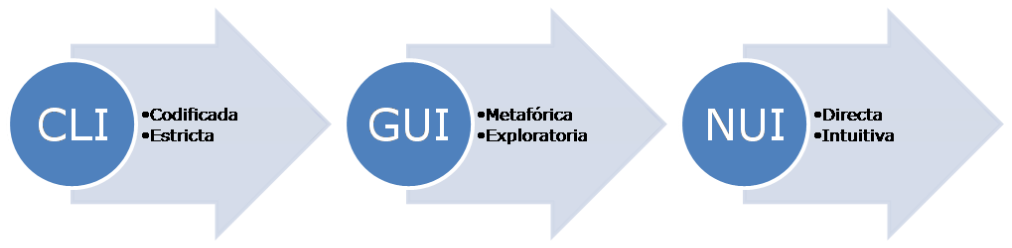
\includegraphics[width=0.7\textwidth]{figures/interfaz.png}
    \caption[Evolución de las interfaces de usuario]%
            {Evolución de las interfaces de usuario \citep{wikipedia4}}
    \label{fig:Evolucion_Interfaz}
\end{figure}

Las interfaces de usuario han evolucionado en diferentes formas de interacción:
\begin{itemize}
    \item CLI (Command Line Interface). El usuario escribe comandos en una consola o terminal.
    \item GUI (Graphical User Interface). Interfaz gráfica con ventanas, iconos y menús, más intuitiva y exploratoria.
    \item NUI (Natural User Interface). Interacción más directa e intuitiva, basada en mecanismos como el tacto, la voz o los gestos.
\end{itemize}

Un buen diseño de interfaz busca usabilidad e intuición, permitiendo al usuario dar órdenes al sistema operativo y visualizar información de estado. 
Esto incluye terminales, escritorios, menús de configuración o iconos de carpeta. El estilo de interfaz puede variar mucho entre sistemas, 
desde texto puro en algunos Unix básicos hasta entornos gráficos completos en sistemas modernos.

\subsection{Seguridad y protección}
La seguridad en un sistema operativo busca garantizar que solo los usuarios autorizados utilicen los recursos y lo hagan de la manera adecuada. 
Uno de los principios fundamentales es el de menor privilegio: cada proceso recibe únicamente los permisos estrictamente necesarios.  
La autenticación permite identificar al usuario, generalmente mediante contraseña, y asignar permisos correspondientes. 
En sistemas como Multics, un servicio de autenticación asocia cada proceso a un usuario; si este servicio falla, un proceso podría recibir permisos indebidos al quedar vinculado con un usuario equivocado~\citep{columbia2008}.

\subsubsection{Control de acceso}
El sistema operativo aplica un modelo de control de acceso que asigna permisos a los distintos recursos (archivos, dispositivos, regiones de memoria, etc.).  
Cada solicitud de un proceso se comprueba mediante un monitor de referencia, que valida las operaciones de acuerdo con los permisos asignados.  
De manera conceptual, esta verificación puede representarse como una matriz de acceso, donde las filas corresponden a procesos o dominios, 
las columnas a objetos del sistema y las celdas a los permisos de lectura, escritura o ejecución.  

En Unix, por ejemplo, cada archivo tiene bits de permiso y un propietario, siendo este último quien puede modificar los bits de acceso del archivo~\citep{columbia2008}.
\subsubsection{Aislamiento de procesos y protección de memoria}
El sistema operativo protege la memoria y el contexto de cada proceso para impedir interferencias entre ellos. Cada proceso se ejecuta en modo usuario (no privilegiado) dentro de su propio espacio virtual de direcciones.  
De esta manera, ningún proceso puede leer o escribir directamente en la memoria de otro, ni en la memoria del núcleo.  
La protección de memoria asegura que los datos de un usuario no puedan ser accedidos por otro y que el código crítico del kernel permanezca intacto.  

Un ejemplo de este mecanismo es la arquitectura de privilegios o *rings*, donde las instrucciones sensibles solo se permiten en modo kernel (nivel 0).  
En este nivel privilegiado se ejecutan las operaciones críticas sobre memoria y dispositivos~\citep{princeton2018}.

\subsubsection{Prevención de intrusiones}
Además de la protección interna, el sistema operativo incorpora mecanismos activos frente a amenazas externas o internas.  
Un sistema de prevención de intrusiones (IPS) supervisa el tráfico y la actividad en busca de comportamientos anómalos, ya sea mediante firmas conocidas o por detección de desviaciones.  
Si se identifica una amenaza, el IPS puede bloquearla antes de que cause daño, por ejemplo cerrando conexiones peligrosas o eliminando contenido malicioso.  

Estos mecanismos suelen incluir filtros y cortafuegos integrados en el sistema operativo, que rechazan accesos no autorizados —ya sea por red o de manera local— según las políticas definidas.  
En conjunto, el sistema previene ataques como virus, intrusiones de red o escaladas de privilegios, al analizar cada petición de acceso y denegarla cuando coincide con patrones maliciosos~\citep{ibm2019}.

\subsubsection{Auditoría y registro}
Con el fin de detectar incidentes y comportamientos sospechosos, el sistema operativo mantiene registros de auditoría de eventos relevantes: inicios y cierres de sesión, errores de autenticación, intentos fallidos de acceso, cambios en permisos, entre otros.  
Cada evento se almacena con la fecha, el usuario y la acción realizada, lo que permite revisar los logs para identificar accesos indebidos o intrusiones después de que ocurran.  

Los sistemas de auditoría más avanzados incluso generan alertas automáticas al equipo de seguridad cuando detectan anomalías en el comportamiento~\citep{ibm2019}.

\subsubsection{Modelos de seguridad clásicos}
En sistemas operativos con seguridad reforzada también se emplean modelos formales que definen con rigor las reglas de acceso.  
El modelo Bell–LaPadula se centra en la confidencialidad, aplicando el principio de “no leer hacia arriba, no escribir hacia abajo” (*read down, write up*).  
Con ello, un sujeto solo puede leer información de igual o menor nivel de clasificación y escribir en niveles iguales o superiores, evitando fugas de datos sensibles.  

Por otro lado, el modelo Biba protege la integridad mediante las reglas opuestas: “read up, write down”.  
Así se evita que un proceso de baja integridad contamine a uno de mayor integridad, o que datos críticos se vean corrompidos por información poco confiable.  

En la práctica, estos modelos, junto con variantes como Clark–Wilson, proporcionan una base sólida para garantizar tanto la confidencialidad como la integridad en sistemas multigrado~\citep{columbia2008}.


\chapter{Revision de S.O. existentes}

\section{Windows}

\begin{figure}[H]
    \centering
    
\includegraphics[width=0.4\textwidth]{figures/logoWindows.png}
    \caption[Ícono de Windows]
            {Ícono de Windows \citep{windowslogo2021}}
    \label{fig:windows}
\end{figure}

Windows es un sistema operativo desarrollado por Microsoft, cuyo origen se remonta a 1985 con la versión Windows 1.0, como una interfaz gráfica que extendía las funciones de MS-DOS. Desde entonces ha evolucionado hasta convertirse en una plataforma dominante en PCs, con múltiples versiones comerciales orientadas a usuarios domésticos, negocios y servidores \citep{Natividad2023}.

Windows posee una arquitectura monolítica, ya que gran parte del núcleo y los controladores E/S del dispositivo se procesan  en modo kernel compartiendo la memoria. Windows es similar al sistema de UNIX, Windows tiene incluido una abstracción de hardware (HAL) y subsistema en modo usuario con el Win 32, POSIX, OS/2. \citep{ Russinovich2005}

Está desarrollado en el lenguaje de programación C con sus componentes de bajo nivel como gestor de memoria, procesos, administración de E/S y partes de la interfaz del usuario y del sistema se implementaron en C++ y en ensamblador para las rutinas más sensibles, como arranque, gestión de interrupciones y entre otros \citep{ Russinovich2005}.

Entre sus componentes clave se encuentran el planificador de procesos y subprocesos que maneja procesos e hilos en modo kernel, el gestor de memoria virtual con paginación que protege cada proceso, subsistemas de archivos como NTFS, soporte de red integral, sistema de drivers para dispositivos hardware, interfaz gráfica de usuario (GUI), componentes de seguridad como control de acceso, y el HAL para manejar diferencias entre arquitecturas de hardware \citep{Forrester2000}.

Windows tiene una comunidad muy grande de usuarios, desarrolladores y empresas. La documentación se publica mediante Microsoft Docs, los libros “Windows Internals” son referencias reconocidas, y Microsoft suele liberar guías técnicas, SDKs y APIs para desarrolladores. Sin embargo, el código fuente no es completamente abierto, lo que limita análisis y ediciones o posibles cambios en el codigo.

\section{Mac OS}
\begin{figure}[H]
    \centering
    
\includegraphics[width=0.3\textwidth]{figures/macOS.png}
    \caption[Ícono de macOS]%
            {Ícono de macOS \citep{GQInfo_macOS}}
    \label{fig:sistema_operativo_mac_os}
\end{figure}
El proyecto Mach dio comienzo en 1985 en la universidad de Carnegie Mellon con la finalidad de crear un microkernel que reemplace al BSD. Su diseño buscaba más seguridad para los usuarios, nose genero lo resultados esperados y se cancelo en 1994. Entonces el proyecto fue adoptado pro OSF/1 Y NeXTSTEP por lo que completo al combinar los componente de BSD, dando origen al kernel XNU de tipo monolítico, pero presento limitaciones con el System 7 y fracaso el proyecto, por ultimo este último avance fue adquirida por Steve Jobs, lo que permitió integrar NeXTSTEP y su kernel XNU como nuevo sistema operativo a Mac OS X, lanzado en 24 marzo del 2001 con el kernel de XNU, que integraba Mach 3.0 y el marco I/O kit, además de ser integrado en Intel Y ARM \citep{Keuper2012}.
El kernel de XNU prosee una arquitectura hibrida que tiene 4 componentes clave \textbf{Mach} que se encarga de administrar las tares, que contine hilos. Su caracteristica principal es la mensajería, mediante puntos de comunicación (IPC), usa el Mach Interface Generator (MIG) para acortar lo procesos, tenemos tambien \textbf{BDS} que implementa procesos y señales UNIX, adema de sistema de archivos y redes, \textbf{I/O Kit} es el marco de controladores orientado a objetos y por ultimo \textbf{KEXTs}  que encargar de enlazar  no solo con el I/O Kit, sino tambien con otras partes del kernel, extensión de red, sistema de archivos \citep{Levin2007}.
Varios de los primeros trabajos de software abierto de Apple son Darwin y WebKit. Darwin es un sistema operativo público que Apple introdujo en el año 2000. Este sistema fue liberado bajo la Licencia Pública de Apple (APSL), que ha sido aceptada por la OSI y la FSF \citep{Levin2007}
\section{Linux}

\begin{figure}[H]
    \centering
    
\includegraphics[width=0.4\textwidth]{figures/linux.jpeg}
    \caption[Ícono de Linux]%
            {Ícono de Linux \citep{wikipedia5}}
    \label{fig:linux}
\end{figure}

Linux es un sistema operativo de tipo Unix iniciado en 1991 por Linus Torvalds como un kernel monolítico, modular y multitarea.  
Originalmente escrito para PCs i386, ha evolucionado hasta ofrecer compatibilidad POSIX y soporte extenso de hardware, siendo desarrollado bajo el modelo de código abierto, donde las mejoras provienen de contribuyentes individuales y corporativos, mientras que la dirección general la marca la comunidad y no un único proveedor \citep{wikipedia5, oci2024}.  
{\sloppy
Su arquitectura se basa en un kernel monolítico moderno que integra características modulares. Todo el núcleo, incluidos los controladores de dispositivos, se ejecuta en un único espacio de direcciones en modo kernel. Sin embargo, soporta la carga y descarga dinámica de módulos en tiempo de ejecución, lo que le otorga flexibilidad similar a la de los micronúcleos sin sacrificar el rendimiento propio de un diseño monolítico \citep[pp.~7]{love2010}.  
}
El núcleo de Linux está escrito principalmente en C, con secciones críticas en ensamblador para optimizar la interacción directa con el hardware. Las aplicaciones en espacio de usuario, en cambio, pueden desarrollarse en diversos lenguajes como C, C++, Python o Rust.  

Entre sus componentes principales se encuentran la gestión de memoria con asignación y protección, la planificación de procesos que regula el uso de la CPU, los controladores de dispositivos para el hardware, el sistema de llamadas al sistema con sus mecanismos de seguridad, y el sistema de archivos virtual (VFS), encargado de unificar múltiples formatos y módulos adicionales \citep{oci2024}.  

Linux posee una de las comunidades de código abierto más amplias y activas del mundo, integrada por miles de desarrolladores pertenecientes a empresas como Red Hat, Google, Intel o IBM, así como por colaboradores independientes. La documentación es igualmente extensa e incluye las \texttt{man pages}, el proyecto de documentación oficial del kernel (\url{https://docs.kernel.org/}), wikis como la Arch Wiki, foros especializados y numerosos libros técnicos.  

\section{MINIX 3}

\begin{figure}[H]
    \centering
    
\includegraphics[width=0.4\textwidth]{figures/minix.jpeg}
    \caption[Ícono de MINIX 3]%
            {Ícono de MINIX 3 \citep{usenix2010}}
    \label{fig:minix}
\end{figure}

MINIX fue creado en 1987 por Andrew Tanenbaum como herramienta docente para la enseñanza de sistemas operativos. En 2005 se anunció MINIX 3, una reimplementación centrada en la fiabilidad y la modularidad, cuyo propósito principal es ofrecer un sistema operativo compatible con POSIX, recuperable ante fallos y adecuado tanto para aplicaciones críticas como para entornos educativos. A diferencia de otros sistemas, fue escrito completamente desde cero, sin incluir código de AT\&T, manteniendo compatibilidad con la versión 7 de Unix y los estándares POSIX \citep[pp.~10]{usenix2010}.  

Su arquitectura está basada en un microkernel muy reducido que se encarga únicamente de interrupciones, gestión básica de procesos y comunicación mediante IPC. Todo lo demás se ejecuta en el espacio de usuario como servidores independientes: controladores de dispositivos, gestor de archivos, gestor de procesos y gestor de memoria. Este diseño multiserver permite que cada componente esté aislado, de modo que un fallo en un servidor no comprometa al sistema completo. Incluso cuenta con un servidor de reencarnación que reinicia automáticamente los componentes defectuosos para mejorar la tolerancia a fallos \citep{csvu2007}.  

MINIX 3 está escrito principalmente en C, con secciones en ensamblador dedicadas a la inicialización del hardware y a rutinas críticas de bajo nivel.  

Entre sus componentes principales se encuentran la gestión de procesos, a cargo de un proceso supervisor que controla creación, terminación y recolección de fallos; la gestión de memoria, donde el microkernel provee segmentación y paginación básica mientras un servidor en espacio de usuario administra la memoria virtual; el servidor de archivos (Mini-FS) con soporte POSIX; controladores de dispositivos que se ejecutan como procesos de usuario aislados; y soporte para interfaces gráficas como X11 o entornos ligeros tipo EDE, siguiendo la tradición Unix \citep[pp.~12]{usenix2010}.  

La comunidad de MINIX 3, aunque más pequeña en comparación con otros proyectos de código abierto, ha tenido impacto en el ámbito académico. Hasta 2010 su web oficial registraba cerca de 1.7 millones de visitas y más de 300,000 descargas de CD \footnote{\url{usenix.org}}. El proyecto participó en Google Summer of Code entre 2008 y 2010, y mantiene recursos como wiki, grupos de discusión y repositorios en GitHub. Su documentación se apoya en el libro \textit{Operating Systems: Design and Implementation} de Tanenbaum (3ª edición), artículos académicos y materiales de congresos, lo que lo convierte en una referencia educativa sólida en el campo de los sistemas operativos.  

\section{RedoxOs}
\begin{figure}[H]
    \centering
    \includegraphics[width=0.3\textwidth]{figures/RedoxOs.png}
    \caption[Ícono de RedoxOS]%
            {Ícono de RedoxOS \citep{WikiRedoxOS}}
    \label{fig:sistema_operativo_redoxos}
\end{figure}
Redox es un sistema operativo tipo Unix que está escrito en el lenguaje de programación Rust, con el objetivo de implementar un microkernel y un sistema de aplicaciones. Rust es un lenguaje enfocado en la seguridad, rendimiento, gratuito y fácil de navegar. Redox se enfocó en la mejora de varios sistemas anteriores que presentaban errores. Uno de sus proyectos es Redox OS. Es compatible con POSIX, y la comunidad está trabajando para escribir la biblioteca libc en Rust, llamada relibc \citep{Saini2018}.

Dado que para los sistemas operativos es muy importante la seguridad, porque los sistemas operativos tienen un alto nivel de abstracción sobre los recursos del sistema, más aún en el caso de que Linux tuviera muchos errores en diferentes bibliotecas ocasionados por la seguridad de memoria. Rust en cambio evita todos esos problemas al tener seguridad de memoria en tiempo de compilación. El kernel de Redox contiene más de 20 mil líneas de código, y su diseño es de alto nivel por eso aún puede tener problemas \citep{Ellmann2019}.

El sistema operativo Redox OS se apoya en un microkernel y está inspirado en el sistema operativo MINIX. Las funciones tradicionales se implementan en kernels monolíticos, como controladores de dispositivo, pilas y el sistema de archivos. Los microkernels son más seguros y ofrecen mayor estabilidad, pero una de las principales desventajas es que el rendimiento que ofrecen no está optimizado para la mayoría del hardware actual \citep{Ritter2019}.

En cuanto a sus componentes clave, Redox OS integra un microkernel responsable de los procesos del sistema, un \textbf{sistema de archivos} implementado en espacio de usuario, \textbf{drivers} que también se ejecutan en espacio de usuario para incrementar la estabilidad, y compatibilidad POSIX que permite correr aplicaciones de otros sistemas Unix. También, añade \textbf{la biblioteca relibc}, escrita en Rust para mejorar la seguridad y la compatibilidad, ademas de \textbf{gestión de memoria} segura que evita vulnerabilidades comunes como los desbordamientos\citep{RedoxOS_book}.
\section{xv6}

\begin{figure}[H]
    \centering
    
\includegraphics[width=0.35\textwidth]{figures/xv6.jpeg}
    \caption[Ícono de xv6]%
            {Ícono de xv6 \citep{pdos2016}}
    \label{fig:xv6}
\end{figure}

xv6 es un sistema operativo educativo inspirado en Unix V6, desarrollado en 2006 por el MIT para su curso de sistemas operativos. Su propósito fue proporcionar un kernel moderno y simple que sustituyera al Unix V6 original, cuya complejidad dificultaba la enseñanza. xv6 sigue de cerca la estructura de Unix V6, pero está escrito en C ANSI y se ejecuta en arquitecturas Intel multiprocesador, convirtiéndose en una herramienta práctica y comprensible para la docencia \citep{pdos2016}.  

Su arquitectura corresponde a un kernel monolítico minimalista, en el que todo el núcleo del sistema operativo se ejecuta con privilegios de kernel, sin separación en servidores independientes. xv6 incluye soporte para multiprocesadores mediante bloqueos y estructuras internas de hilos, aunque carece de controladores de red o capacidades gráficas avanzadas. Sus componentes básicos abarcan la planificación de procesos con un esquema round-robin, la gestión de memoria con paginación simple, un sistema de archivos inspirado en Unix V6 y un conjunto reducido de llamadas al sistema \citep[pp.~25]{mit2022}.  

La implementación de xv6 está escrita principalmente en C, mientras que el código de inicio y las rutinas de interrupción se desarrollan en ensamblador x86. En sus versiones más recientes, también se encuentra una adaptación para la arquitectura RISC-V, lo que amplía su aplicabilidad en contextos educativos.  

Entre los componentes principales destacan la gestión de procesos, que otorga a cada uno su propio espacio de direcciones, con un planificador round-robin y un cambio de contexto sencillo; la gestión de memoria mediante paginación básica y un asignador simple para el kernel; un sistema de archivos con inodos y directorios inspirado en Unix V6; y mecanismos elementales de sincronización como \texttt{sleep} y \texttt{wakeup}, que permiten estudiar las condiciones de carrera. Además, xv6 expone llamadas al sistema tradicionales de UNIX como \texttt{fork}, \texttt{exit}, \texttt{wait}, \texttt{open}, \texttt{read}, \texttt{write} y \texttt{close}, lo que facilita comprender la implementación exacta de estas primitivas fundamentales \citep[pp.~26--30]{mit2022}.  

xv6 se ha consolidado como una herramienta académica ampliamente utilizada en universidades para cursos de sistemas operativos. Su código fuente está disponible públicamente, y los propios autores distribuyen un libro titulado \textit{xv6: a simple, Unix-like teaching operating system}, que comenta línea por línea el código y explica tanto el funcionamiento como el diseño de sus estructuras y funciones. Gracias a su claridad y abundante documentación, xv6 se ha convertido en uno de los sistemas operativos de referencia para la enseñanza de fundamentos prácticos de diseño de kernels \citep{mit2022}.  

\section{FreeRTOS}
\begin{figure}[H]
    \centering
    
\includegraphics[width=0.3\textwidth]{figures/FreeRTOS.png}
    \caption[Ícono de FreeRTOS]%
            {Ícono de FreeRTOS \citep{img_FreeRTOS}}
    \label{fig:sistema_operativo_FreeRTOS}
\end{figure}
FreeRTOS es un sistema operativo en tiempo real con un kernel planificador, desarrollado para ejecutarse con microcontroladores. Está compuesto funcionalidades de planificación en tiempo real, comunicación entre tareas, análisis temporal y primitivas de sincronización con el propósito de cumplir con las tareas con el plazos estrictos de ejecución \citep{He2020}.
En cuanto a su arquitectura hace uso de un microkernel para administrar tareas en tiempo real, casi similar al RTLinux en que admiten núcleo dual, lo que permita separar tareas critica y no criticas \citep{Serino2019} Esta escrito en lenguaje C estándar y con algunas lineas de código en ensamblador para que se acople a diferentes arquitecturas.
Dentro de su componentes claves tenemos el \textbf{planificador}, \textbf{mecanismos de comunicación}, \textbf{sincronización} gracias al uso de colas y semáforos. Incluyendo la estructura de \textbf{Task Control Block (TCB)} para la administración de procesos y tareas \citep{Barry2018}.
\begin{figure}[H]
    \centering
    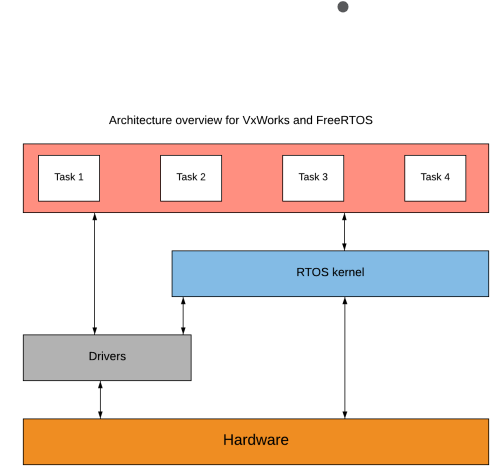
\includegraphics[width=0.3\textwidth]{figures/ArquitecturaFreeRTOS.png}
    \caption[Arquitectura de FreeRTOS]%
            {Diseño de la arquitectura de FreeRTOS \citep{img_FreeRTOS}}
    \label{fig:Disenio_operativo_FreeRTOS}
\end{figure}
FreeRTOS es código abierto con una licencia GPL, lo que permite su uso en aplicaciones comerciales. El código está disponible públicamente y cuenta con documentación extensa en el código fuente en su sitio oficial \citep{FreeRTOS_org}.
\section{Fuchsia}

\begin{figure}[H]
    \centering
    
\includegraphics[width=0.35\textwidth]{figures/fuchsia.jpeg}
    \caption[Ícono de FuchsiaOS]%
            {Ícono de FuchsiaOS \citep{fuchsia2025}}
    \label{fig:fuchsia}
\end{figure}

Fuchsia OS es un sistema operativo desarrollado por Google desde 2016, diseñado como una plataforma de propósito general para dispositivos embebidos, móviles, IoT y potencialmente de escritorio. A diferencia de Android, no se basa en Linux, sino en un núcleo propio denominado Zircon \citep{zirconkernel}.  

Su arquitectura está basada en un microkernel, en el que Zircon gestiona procesos, hilos, memoria y comunicación mediante objetos e IPC, mientras que servicios como sistemas de archivos y controladores se ejecutan en espacio de usuario, favoreciendo la seguridad y modularidad \citep{fuchsiadocs}.  

Fuchsia está escrito principalmente en C++, Rust y Dart. Zircon se implementa en C/C++, mientras que la capa de interfaz gráfica se desarrolla con Flutter (Dart), lo que facilita la portabilidad a múltiples plataformas \citep{googlefuchsia}.  

Entre sus componentes clave se encuentran la gestión de procesos basada en objetos, memoria virtual con aislamiento estricto, soporte para múltiples sistemas de archivos (como MemFS, BlobFS y FAT) y un entorno gráfico con Flutter para experiencias multiplataforma \citep{zirconkernel}.  

El proyecto es mantenido principalmente por Google, con participación de la comunidad de código abierto. Su documentación oficial está disponible en Fuchsia.dev, que incluye guías técnicas, API y manuales de contribución, aunque parte del desarrollo se mantiene cerrado \citep{fuchsiacommunity}.

\section{Haiku}

\begin{figure}[H]
    \centering
    
\includegraphics[width=0.35\textwidth]{figures/haiku.jpeg}
    \caption[Ícono de HaikuOS]%
            {Ícono de HaikuOS\citep{haikuos2025}}
    \label{fig:haiku}
\end{figure}

Haiku es un sistema operativo de código abierto inspirado en BeOS, iniciado en 2001 con el objetivo de proporcionar un entorno moderno, rápido y sencillo de usar, orientado principalmente a equipos de escritorio \citep{haiku2025}.  

Su arquitectura es híbrida, ya que utiliza un núcleo monolítico modular, pero con elementos que recuerdan a un microkernel, lo que equilibra rendimiento y flexibilidad \citep{haikudevdocs}. El sistema está desarrollado principalmente en C++, con partes en C y ensamblador para las interacciones de bajo nivel \citep{haikudevdocs}.  

Entre sus componentes clave se incluyen un modelo de multitarea preventiva con planificación por prioridades, gestión de memoria virtual con paginación y aislamiento de procesos, y un sistema de archivos propio llamado OpenBFS, optimizado para indexación rápida \citep{haikufs}. Además, cuenta con una interfaz gráfica uniforme gestionada por el app\_server.  

Haiku es mantenido por la Haiku Project Foundation y su comunidad de desarrolladores voluntarios. El proyecto dispone de documentación oficial, foros y repositorios activos en GitHub, con lanzamientos beta periódicos que permiten probar y evaluar su madurez \citep{haikucommunity}.

\section{ToaruOS}

\begin{figure}[H]
    \centering
    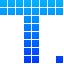
\includegraphics[width=0.4\textwidth]{figures/logoToaruOS.png}
    \caption[Ícono de ToaruOS]
            {Ícono de ToaruOS \citep{toaruoslogo2025}}
    \label{fig:ToaruOS}
\end{figure}

ToaruOS creado en 2010 por Kevin Lange, es un sistema operativo experimental con fines educativos, que busca evidenciar cómo se puede desarrollar un entorno completo desde la nada, independiente de kernels o librerías existentes. Su intención primigenia fue servir como soporte de investigación y aprendizaje para la comprensión del formato y funcionamiento interno de un sistema operativo moderno, incorporando subsistemas gráficos, de red y de usuario. A diferencia de proyectos como Linux o BSD, ToaruOS busca ser un entorno accesible para la enseñanza y la experimentación, y no un sistema de producción \citep{toaruos2025}.

La arquitectura de ToaruOS es híbrida. Esto significa que el kernel es en gran medida monolítico por lo que, incluye directamente los módulos significativos del sistema, como la administración de memoria, procesos, controladores de dispositivos y el sistema de archivos, pero incluye características de microkernel como la posibilidad de ejecución modular. Este diseño posibilita la integración y el rendimiento en un entorno practico. El lenguaje de implementación es C, con cantidades inferiores en ensamblador para interrelaciones de bajo nivel con el hardware y el arranque \citep{toaruos2025}.

Los elementos nucleares del sistema comprenden los elementos básicos de cualquier sistema operativo contemporáneo. Para la gestión de procesos pone en práctica tareas múltiples planificadas basada en prioridades, de igual manera de resistir hilos ligeros. Para la gestión de memoria abarca paginación, segmentación y asignación dinámica de memoria para los programas de usuario. Al respecto del sistema de archivos, dispone de su peculiar implementación denominada “tmpfs” para sistemas en memoria, asimismo la compatibilidad con EXT2 en versiones más actuales. Por otra parte, cuenta con un sistema gráfico completo, compuesto por un servidor de ventanas (Toaru Window Server), un gestor de ventanas y librerías gráficas que permiten ejecutar aplicaciones con interfaces gráficas, como un editor de texto o un navegador web básico \citep{toaruos2025}.

La comunidad de ToaruOS es reducida en comparación con otros proyectos de código abierto, pero se mantiene activa en torno a su repositorio en GitHub, donde se documentan los cambios y se comparten implementaciones experimentales. La documentación disponible proviene principalmente de su creador, quien mantiene guías, el repositorio en Github y un blog explicativo sobre su evolución. Se ha mencionado grosso modo en limitadas ocasiones en artículos científicos de especialidad.
\chapter{Comparación técnica}

La tabla siguiente presenta una comparación técnica de varios sistemas operativos destacados, considerando aspectos clave como arquitectura, lenguaje de programación, tamaño del kernel, soporte de hardware, documentación y comunidad de usuarios y desarrolladores.

\begin{sidewaystable}[p]
\centering
\caption{Comparación resumida de distintos sistemas operativos en orden de popularidad, elaborada en base a la investigación realizada en este proyecto.}
\vspace{0.5cm} 
\begin{tabular}{|c|c|c|c|c|c|c|}
    \hline
    \textbf{Sistema} & \textbf{Arquitectura} & \textbf{Lenguaje} & \textbf{Kernel} & \textbf{HW} & \textbf{Documentación} & \textbf{Comunidad} \\ 
    \hline
    Windows & Monolítica & C++ & Grande & Amplio & Excelente & Masiva \\ 
    \hline
    XNU & Híbrida & C++ & Grande & Intel & Buena & Apple \\ 
    \hline
    Linux & Monolítica & C & Grande & Amplio & Excelente & Activa \\ 
    \hline
    MINIX & Microkernel & C & Pequeño & Limitado & Buena & Académica \\ 
    \hline
    Redox & Microkernel & Rust & Mediano & Limitado & Moderada & Experimental \\ 
    \hline
    xv6 & Monolítica & C & Pequeño & Limitado & Excelente & Académica \\ 
    \hline
    FreeRTOS & Microkernel & C & Minúsculo & Amplio & Extensa & Embebidos \\ 
    \hline
    Fuchsia & Microkernel & C++ & Mediano & IoT & Buena & Google \\ 
    \hline
    Haiku & Híbrida & C++ & Mediano & Limitado & Buena & Constante \\ 
    \hline
    ToaruOS & Híbrida & C & Pequeño & Limitado & Básica & Reducida \\ 
    \hline
\end{tabular}
\label{tab:comparacion_so_custom_h}
\end{sidewaystable}


%\printbibliography
\clearpage
\phantomsection   
\addcontentsline{toc}{chapter}{Referencias}
\bibliographystyle{apalike}
\bibliography{ref}

% If you have no appendices, remove the following two lines.
% If you have more appdences, add them as necessary.
%\appendix
%\include{apdxa}

\end{document}
